

\section{Approach}
The task of speaker recognition can be considered as a task of classification. Thus a number of machine learning techniques
can be applied to this task. In general, this task should cover the following three topics:

\begin{enumerate}
  \item Feature Extraction: process the voice signal and extract acoustic features that
	  could describe the acoustic characteristics of speakers, which can be correlated
	  in some extend to model latter used.

  \item Acoustic Model: provide the functionality of registration as well as identification or verification.

  \item Evaluation: Evaluate our approach using datasets with appropriate metrics.
\end{enumerate}

\subsection{Feature Extraction}
The task of speaker recognition is highly correlated to the task of speech recognition.
In the field of speech recognition, Complex Cepstrum \cite{cepstrum} is
considered to be a concise description to the original acoustic signal.
In particular, Mel-frequency Cepstral Coefficients (MFCC), is a state-of-the-art standard feature
widely used in Automatic Speech Recognition (ASR) system.
The general procedure for calculating MFCC is as follows:
\begin{figure}[H]
  \centering
  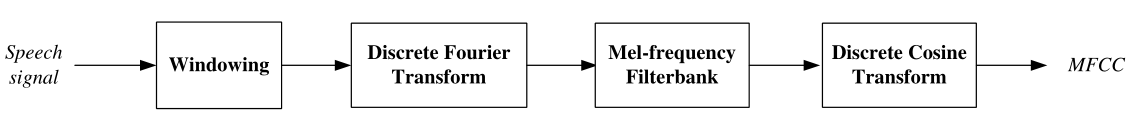
\includegraphics[width=\textwidth]{res/MFCC.png}
\end{figure}

As for speaker recognition, several different features are suggested and compared
by researchers \cite{evaluation}. Cepstrum still proves to be a robust and effective
feature in this task. Therefore, a bunch of cepstral features, including MFCC,
LPCC (Linear Prediction Cepstrum Coefficients), are commonly used
in speaker recognition system.\cite{feature}

We plan to implement common cepstral features used by researchers, and use a
combination of some of them, according to the further observation and test on how
much they contribute to the task.

\subsection{Model}
According to works in years, Gaussian Mixture Model (GMM)
has been a common approach to acoustic modeling.\cite{GMM}
GMM can be used to acquire an acoustic model $P(\mathbf{O} | \mathbf{W}) $,
which gives the probability of a given observation
$\mathbf{O}$ under certain word $\mathbf{W}$. By using GMM, this
conditional probability can be well estimated by modeling the distribution as
a sum of several normal distribution.

In addition to that, Hidden Markov Model (HMM) is a main-stream approach in ASR system,
since it can describe sequential relation of observations.\cite{SLP}
We have noticed a few research-oriented open-source speech recognition
tool building on HMM, such as HTK\cite{htk}.
Such tools might be quite useful in buiding a speaker recognition system.

Recently, some common machine learning model are also applied to the task of speaker
recognition. \cite{svm} suggested a method of using SVM in speaker recognition.
Deep neural networks are also used in speech processing recently.\cite{deep}

HMM and GMM will probably be our first attempt, as they are already widely used and proven to be
efficient and effective.  We might also try to migrate our extracted feature to
some other available models.

\subsection{Evaluation}
\subsubsection{Dataset}
There are a number of well-known databses for speaker recognition system evaluation,
such as KING speaker verification\cite{king}. \cite{database} gives description on
several common databases. But most of these databases are not free of charge.
We intend to search for an freely available database,
otherwise we have to build some simple test cases by our own.
\subsubsection{Metrics}
As we intend to distinguish different speakers, the primary goal is overall
accuracy of the system we built. Furthermore, the performance may differ from
speaker to speaker, which may provide with additional feedback to our approach.
Thus we shall examine precision, recall and $F_1$ score for each speaker.

